\documentclass[portrait,a4paper]{article}
\usepackage[no-math]{fontspec}
\usepackage{xeCJK}
% \setCJKmainfont[BoldFont=SimHei,ItalicFont=TW-Kai]{SimHei}
% \setCJKmainfont[Scale=1.5,Script=CJK,Vertical=RotateGlyphs]{SimHei}
\setCJKfamilyfont{songvert}[RawFeature={vertical},Scale=1.6,Script=CJK,Vertical=RotatedGlyphs]{SimHei}
% {AR PL KaitiM GB}
% \setCJKfamilyfont{songvert}[Script=CJK,Vertical=RotatedGlyphs]{SimSun}
\xeCJKsetup{CJKecglue = {\hskip 0.2em plus 0.02em minus 0.01em},
	xCJKecglue = {\hskip 0.2em plus 0.02em minus 0.01em}}

\usepackage[a4paper,margin=0.5in,footskip=0.2in]{geometry}

\usepackage{everypage}
\AddEverypageHook{\special{pdf: put @thispage <</Rotate 90>>}}

%\usepackage{zxjatype}
%\usepackage{flowfram}
%\newflowframe{\textheight}{\textwidth+2em}{0pt}{\textheight}[mainframe] 
%\setflowframe{1}{angle=-90} 

\usepackage{parskip}
\setlength{\parskip}{1em} % 1ex plus 0.5ex minus 0.2ex}
\lineskip=0.5em

\title{真的,好恐怖}
\author{岩井志麻子 (1999)}
\date{}

\begin{document}
\maketitle

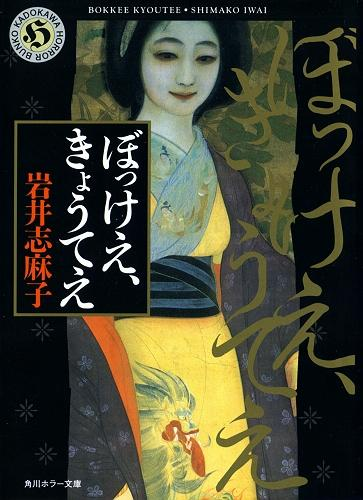
\includegraphics[scale=1.0,angle=90,origin=c]{cover-真的,好恐怖.jpg}

——您做噩梦了吗?

……是梦到了什么呢。喔,是在睡梦中梦到那个啊。原来是那个啊。

我说老爷,您怎么像个孩子一样呢。不不不,我不会嘲笑您的。毕竟所谓的做梦,通常都会非常恐怖不是吗。

您问妾身?妾身呀……光是清醒时所看到的东西,就已经够恐怖的了,所以入睡后反倒什么都看不见。

妾身的梦总是一片漆黑。伸手不见五指。连我自己都想不起究竟梦见了什么。

老爷,请您放心的睡吧。您瞧,还吹来了一阵凉风呢。尽管没装蚊帐,但只要像这样用扇子一直扇啊扇的,蚊子就不会来了。

只要妾身醒着,什么妖魔鬼怪都不敢来的,所以请您快点闭上眼睛吧。

妾身不能让老爷您看到我的睡颜。被客人看到睡着后的容颜,可是青楼女子的最大耻辱呀。

不是有人说,青楼女子绝不仰卧入睡,只能面向右方侧躺的吗。虽然许多妓女偶尔会呈现大字型入睡,但是妾身从不会如此失态。

从孩提时候开始,妾身都是面向右侧入睡。

您说,所以妾身的脸才会长成这样吗?呵呵呵,老爷您真讨厌耶。

妾身的眼睛跟鼻子,的确往左边太阳穴的方向歪斜。因此,嘲笑妾身是丑女的顾客大有人在,被妾身的长相吓到的客人也不在少数。

应该是有只看不到的手将妾身的五官往左上方拉扯吧?所以,恐怖的好像不是妾身这张脸,而应该是那只手吧。

您说,看不到的东西才恐怖?可是,妾身觉得双眼可见的东西也是恐怖至极呀。

那是因为……算了,别说了。如果真说给老爷您听,只怕您真要睡不着了。妾身这并不是要威胁您,而且往后也不会的。

对了,自古流传一句话,名妓必须具备一容貌二床功三手技。妾身却是三项都缺。诚如您所看到的,面貌丑陋又不讨人喜欢。

即便没有镜子,妾身也能清楚看透自己的长相。不只是妾身自己的长相,就连普通人看不到的东西,妾身也能看得一清二楚。

其实,妾身的年纪还不算老喔。真的不骗您。在妾身出生那年,那一带还不叫冈山县,而是叫做是北条县呢。是明治九年合并的呀?老爷您果然学识渊博。您说您毕业于高等师范学校?真是了不起。哪像妾身我们这种人,连普通学校或稍微搬得上台面的地方都没去过。

但是妾身并不在意。因为吃饭讨生活这种事,无论猫狗或大字不识的妓女,都是不用教就会熟练的,呵呵呵。

不过,妾身坚持不让客人看到睡颜这件事,为妾身得到礼仪端庄的好评喔。但妾身并不清楚,妓女礼仪端庄能得到什么好处就是了。

所以,老爷您就安心入睡吧。若是又做了梦见什么怪东西的噩梦,妾身会把它们赶跑的。因为妾身很擅长对付妖魔鬼怪呀。

话说回来,老爷您来得有点晚喔。挑选货色在十二点时就结束了。若是黄昏时分前来,便可透过格子窗选妓,各色年轻貌美的妓女任君挑选。但现在就只剩妾身这种卖不掉的丑女,真是对不住您啊。

而且,每个妓女都隔着格子窗,使出浑身解数来赢取客人欢心,只有我蜷曲在角落里吧。

不论老鸨们多么生气的教训我,妾身也绝不从格子窗伸出手去。并不是我爱摆架子,或是态度敷衍草率……我只是觉得好恐怖呀。

因为有些不吉的东西,会来抓住我的手呀。不管是死去的父亲,或是被杀害的朋友等。反倒是那些还活着的男人们,很少会主动来拉我的手。

而且似乎有股微妙的力量,从左侧不断拉扯着妾身的脸。

您说您正是中意我这奇怪的地方吗?老爷您可真是个怪人耶。

可是啊,老爷我跟您说。其实妾身从未被温柔对待过,您这样反而让我感到难受耶。所以,请您千万不要对我说,喜欢我或中意我这样的话。毕竟妾身是个无论到哪都该被残酷对待的女人啊。

……您希望我说点话让您好入睡吗?这当然没问题,但是该说些什么才好呢。既不能说大老板与老鸨的坏话,也不能乱说朋友或其他恩客的闲话。这样一来,就没什么好说的了。

妾身自从十六岁时被卖到这里后,外出的次数可说用手指头都数得出来。而且所谓的外出,就仅止于在夜里透过格子窗仰望天空,或是像今晚这样从二搂的窗口往下望而已。

……您说您想听听妾身的生平?这下子,妾身更加觉得您是个与众不同的客人了。只不过如此一来,好梦将会离您更加遥远唷。

因为只要您听了妾身的生平,就等同于是做了一场恐怖至极的噩梦。

这样也不打紧吗?既然如此,那我就说喽。首先呢,妾身是出生于津山附近,大约离这里六里远的小村庄……至于村名嘛,说了您大概也不知道吧。

那里叫做日照村,俗称强诉谷。村人都以务农为生,但鲜少有丰收年份,总是歉收居多。因此男人多以受雇领日薪的农工身分来糊口,而女人则几乎都远走他乡谋生。被卖到青楼去的也不少,但并非像妾身一样在附近而已,而是被卖至遥远的九州或大阪等地。

一提到冈山,大家总会想到南方那一带,而不禁投以羡慕的眼光吧。土地肥沃,城镇发展迅速,商旅来往也热闹繁荣,造就了许多富有人家。而且……冬天气候也很温暖吧。但我不大喜欢备前那边的人,因为他们都爱要小聪明。什么!老爷您是备前人呀,那还真是失礼了,请原谅我的失言。

……然后呢,再说到我所居住的,那北到不能再北,位于中国山脉最尾端的小村落,可就连半个有钱人都没有,全都是一贫如洗的穷人。即使是十六、七岁的年轻人,脸上跟手脚也全都布满小皱纹而且晒得黝黑无比。能够活到四十岁就已经算是长寿了。

其中最贫穷的人家,就是我们家了。并非我夸大其词,真的是过着连牛都不如的日子。

因为妾身我是饿死仔呀。没错,就是闹饥荒。因为我出生于闹饥荒的年度,所以是饿死伃。

我刚才不是说过,那一带鲜少有丰收,而且每隔一年就会闹饥荒的嘛。

因此,妾身对于死人的记忆远比对于活人要来得多。

不用说,那些当然都不是美好的记忆。不值钱的人命就像草芥一样,死再多也不足惜呀。

我娘是个产婆,但却是个专门帮忙打胎的产婆。

她从未接生过活婴,所以应该连产婆都称不上吧。

村里的人都叫她堕子婆或刺子婆。甚至还有些小鬼们会毫不客气的叫她鬼婆。如此一来,妾身当然就是鬼之子喽。

我们家虽然遭到全村人的排挤,但唯有那个时候才会被村人叫去。

那个时候,也就是指打胎的时候。有时必须把胎儿从孕妇肚子里硬拉出来,有时必须把出生的活婴给闷死。唯有那种时候,我们才有机会与村人打照面。

妾身从四岁开始,就跟在我娘身旁帮忙了。

小时候,我负责去摘采野菊或酢浆草,还有搓麦秆,长大之后……则是负责压住产妇的手脚。工作性质就好像是刽子手的帮手一样。

那些女人们,不怨恨像只母狗般动不动就怀孕的自己,也不怨恨把胎儿拖出来再闷死的我娘,却把那份怨念都移转到我身上……真是令人受不了。

您应该不知道吧?野菊跟酢浆草的根,是用在这个洞的。老爷您方才也用过的呀,呵呵呵,就插进这个洞里,用尖端刺向胎儿好让他流出来。

明明脸跟手脚都被晒得又脏又黑的,但为何那些女人的大腿却那么地白皙肥软呢。不管是多么干扁的女人,大腿上全都装满了肥滋滋的丰润脂肪。

被拉出来的胎儿,皮肤首先会呈现白色,接着转变成鲜血般的红色,临死前则变成暗黑色。

这个洞连接着地狱,妾身从小时候就知道了。

我常想,为什么不把这个洞给封起来呢?万万没想到自己后来居然用这个洞来做买卖。总之,幸好当初没有把它封起来,呵呵呵。

男人并不是性好女色或是喜欢女人的洞,而是喜欢那直通的地狱吧。因为那是他们在出生前所待的地狱呀。

也因此,我从懂事以来,就开始协助杀人的工作。

倒也没有特别开心或难受的感觉,因为这是妾身与生俱来的命运啊。

甚至有人得意洋洋地说:就是因为你杀婴所以那张脸才会长得那么歪斜吧。

我并不会害怕啊。因为……婴儿跟小产儿都是我的好朋友呀。

打胎的工作在饥荒时期反倒生意兴隆。野菊几乎荒芜殆尽。而因草木贫瘠而消瘦的蜻蜒及瘦鸟,来回飞舞于田野间的情景,至今仍鲜明烙印在我的脑海里。

咬紧牙关捱过饥荒的我,也是瘦到与骸骨无异。饥饿的村民们纷纷到附近的山谷挖掘蕨类果腹。即使女人们全都瘦得皮包骨,但是小产儿仍不断增加。因为无论多么饥饿,人们还是无法停止做那档事。

然而,在这么枯寂贫乏的景色中,为何天空会如此澄净湛蓝呢?晶莹剔透到理应看不到的星星似乎也都清晰可见。

关于妾身孩提时期的回忆,除了打胎之外别无其他。那是我小时候的唯一回忆。

将胎儿引产之前,必须先让粪便排出。鲜血与粪便的味道充斥家中,在夏季尤其令人难受。不过,只要把它当作是堕入屎尿地狱前的准备,应该就不足为奇吧。

将粪便装在盆里,然后再将死胎扔进里面。真的是毫无慈悲心的用力一扔。虽说是死去的胎儿,但所受到的待遇却与粪便血块完全相同。

我曾在庙里的地狱草纸上看过描绘着同样情节的画作。绘画的技巧虽然拙劣,却也因此让人感到格外恐怖。

和尚说那张画上的血是真的。但那应该是骗人的吧。怎么可能会有那种永远都保持鲜红色的血呢?血是又黑又臭的东西啊。

话说回来,那小产儿明明什么坏事也没做过,为何会被打入屎尿地狱呢。佛书上不是说,他们既不会下地狱,也无法前往极乐世界,只能在赛之河原哭泣而已嘛。

那个和尚还告诉我,那也是将不洁之物视为洁净,或将洁净之物视为不洁之人所坠落的地狱。可是他也玩弄了妾身的身体呀。那他会坠落到第几层地狱去呢?

那小产儿是因为眷恋着把自己当作粪便丢弃的爹娘,才会无法脱离苦海吧!

即使在现世无法与爹娘见面,在屎尿地狱里应该就能和他们相逢了吧。然而,他爹娘就算在那里,也依然会对自己的孩子视而不见吧。尽管如此,孩子却仍对爹娘恋恋不舍。

……您问妾身为何没被打掉呀?

啊哈哈哈,老爷您府上一定是富贵人家,而且您又是男丁,想必是在众多期待下诞生的吧。您应该是在豪华的宅院里,由温柔的产婆接生下来的吧。

妾身则完全不同。我娘当时已年过四十,而且家中穷到连一只老鼠都没有。

更何况妾身还是个女的。

而且另一个也是女的。没错,我们是双胞胎。可说所有打胎的条件都齐备了。顺带一提,妾身姐姐的外貌也是非比寻常。

……您问到底长啥模样呀?就请您饶了我吧。因为她毕竟是我的姐姐。说出来就太可怜了。

不过,妾身并不是被用野菊根引产出来的,而是顺产生下来的。方才我也提过,那一年适逢饥荒,到处都有女人需要打胎,我娘忙得不得了,一直到足月前都没留意到自己的肚子。

我娘自己一个人生产,还自行清理胎盘,甚至连丢弃婴儿的工作……都自己包办。

总之,她用湿布压住婴儿口鼻,将婴儿扔进了家门前的那条河里。因为那条河是专门用来丢弃小产儿的河川。在理应是蛙鸣不断的夏夜里,那里却是小产儿的哭声不断,而且那哭声是全年无休。

尽管如此,妾身却是毫发无伤。经过了两天依然存活着。

我仍清楚记得在那条河里的那两天……如果我这么说的话,您一定会气我爱说谎吧。但这是千真万确的呀。我的眼睛还睁不开,一直处于幽暗的状态。河水柔软滑溜,飘来一阵女人的气味。妾身没有溺水,也没被乌鸦给吃掉,只是被冲到草丛里去了。

幽暗薄暮的那端,聚集了许多人。轻抚我额头的,应该是被供奉在附近山里的神仙吧。帮我赶走乌鸦的,应该是在临死前大哭一声的某个陌生婴儿吧。不知从何处飘到我嘴边的半腐烂小产儿,则是养分供给者,妾身靠着舔舐他的手脚才得以存活。

我娘在产后隔天即恢复接生工作,当她将被闷死的小产儿拿到河边丢弃时,无意间发现了一息尚存的妾身。

或许是天意吧,这让我娘不由得心生怜惜。

……算了吧,再说下去就太恐怖了。妾身是如此,妾身的姐姐也一样。

您问我姐姐呀?她……已经没了啦。所以,我们就不要再提她了吧。

诚如方才我所说,当时有许多女人还来不及打胎就直接生了。

至今我仍清楚记得,有个婴儿在出生时只有巴掌大小,却已能张开眼睛,嘴巴也能开阖,但还不会哭泣。眼皮都还没长齐全,眼珠却已能滴溜转……眼睛瞪得好大。

他并不是在看妾身或我娘,而是生下他的母亲。但那并不是眷恋不舍的眼神。不过,我娘随即一脚将他踩烂,包进布包里就是了。

您问那个女人吗?您以为她会因此感到懊悔而祭拜小产儿……是吧?我说老爷,您果然是出身于富贵人家喔。

我从未看过因丢弃婴儿而难过哭泣的女人。她们通常都在止住失血之后,便立刻又对那档事狂热不已。然后,再度毫不在意的来找我娘。

这也没办法啦。因为老百姓的生活乐趣,就只有吃饭跟那档事而已啊。

妾身虽然在吃方面相当拮据,但对那档事却未曾烦恼过。呵呵呵,这大概可说是天赐的诅咒吧。因为妾身即使没做防范措施也不会怀孕哟。我们妓院里,有个被叫做畜生肚、像母狗般动不动就怀孕的女人,但妾身却从不曾怀孕过。

我想,大概是因为妾身……仍然跟个小产儿一样吧,哇哈哈。

话说回来……不知那些小产儿在死前看到的是什么样的世界?我想,即使他们看到了,大概也料想不到那就是现世吧。

他们八成以为自己又回到了地狱吧。因为映入他们眼帘的,就是堕子婆跟她女儿,以及生下自己的母亲这三只鬼啊。

呵呵呵,说好要让您做个好梦,却将您引到做噩梦的方向。难道这是天谴吗?下次请让擅长床第之术的美女来服侍您吧。

什么……您很在意为何我家会遭到全村隔离啊?我说老爷,您还真是喜欢听鬼故事呀。您该不会是想做噩梦吧。

好吧,那妾身要开始说喽。虽然说来话长,但刚开始大概是因为我们是外来者吧。那个村庄的愚夫愚妇们对于在中国山脉的对面,住着三只眼的孩子、长角的男人,以及私处往两旁裂开的女人这类的传说,深信不疑。因此,对于外来者都避之唯恐不及。

我说过我爹跟我娘都是出身于四国吧。他们因为在四国老家没有容身之处,所以才逃到冈山来的。假行脚之名,行乞讨之实,一路流浪到了津山。

您问我为什么难以容身?这个啊,就算了吧。妾身也是有难言之隐的呀。

……老爷,虽然您从刚才就不断抱怨这房子太简陋了,但是依妾身看来,这里简直可媲美冈山城啊。因为妾身所住的老家,原本是牛棚呀。

妾身被卖到这里后,才第一次看到榻榻米。天花板也是首次看到。尽管妓女跟牛马一样卑贱,但好歹都还人模人样啊。妾身是在被卖到这里之后,才开始活得像个人一样。即使没有棉被,妾身也能蜷曲身子就地而眠。因此,我才能像现在这样,轻松自在的上夜班哪。反倒是仰卧入睡,让我觉得好像有股风直往胳肢窝里吹,令人感觉寒冷。

在那一带,每到夏天便有北风来袭。风势强劲得有如龙卷风般,经常一口气便将好几片屋顶给吹飞了。

我们所住的地方,后面有座山,门前有条河。而冥界与现世的分界,其实不只存在于阴间,我家门前也有一条。因为那山里到处可见饿死尸,而河里则是布满小产儿。

在河流的前方,就是村民们的田地。尽管那是片寸草不生、碎石遍布的贫瘠田地,但也够令人羡慕的了。我家连块地也没有。如果有的话,我就不会被卖到这里来了。

我爹是个受雇领日薪的小农夫。虽说寻常百姓根本不需要任何学问,但我爹还真是个一无是处的人。居然连算术都只能算到五。

我爹不爱干活,总是看心情决定去上工或不去上工。偶尔领到钱,也全都花在买醉上头。

更何况那里的气候非常恶劣,农作物经常歉收。妾身跟我娘只得靠着残杀胎婴挣钱过日子。唉,真的是困苦到只剩一口气呀。

尽管如此,每当看到北风无情摧残村民们的田地时,妾身总是非常开心。并不是我幸灾乐祸,而是那景致太美了。

金黄色稻穗遭到黑压压的北风肆虐,简直就像厉鬼从山上降临,而在沿路留下了足迹。而那足迹,总是不知不觉在我心中消失。

因为只有妾身才看得见那只鬼呀……他是个相当不错的男人哟。只不过输老爷您一大截就是了,呵呵。

话说回来,每到夏天,我家屋里屋外就会臭到令人受不了。河里经常有小产儿的尸体,载浮载沉而日渐腐烂,不久就会变成小尸骨了。

最不可思议的是,在那些变黑发臭还不断膨胀的死尸里面,居然还有活着的小生命。绝对不是我眼花喔。因为那个小产儿还会讲话呢。

您问我他说了什么话?这个嘛……我不太想说耶。反正不是什么好话就是了。

老爷您知道魔界之路吗?就是妖魔鬼怪所通行的道路。那原本是尊贵神明的使者所往来的通道,却因使者们的信念不坚,而化成了可怕的场所。

村民们不只在提到我家时会压低声量,就连说到那片土地时也一样。

我家就住在魔界之路的正上方呀。所以啊,所有忌讳不祥的条件全都具备了。但妾身家完全不在意。因为再也没有比这更惨的事情了。

……爹娘希望我能外出谋生,但感谢上天眷顾,没有地方愿意雇用我。妾身的朋友,就只有那些在河里腐烂的胎婴死尸而已。因此,我经常跟他们玩家家酒的游戏。

附近活着的小鬼头们很令人讨厌,但死掉的婴儿却很惹人怜爱。尽管眼睛嘴巴都还没长全,但感觉纯真又乖巧。

不过,即使我还帮喜欢的小产儿取名字并疼爱有加,但他们马上就腐烂成骨了。其中也有那种不知为何都不会腐烂、令人感到不可思议的婴儿哟。那是个在娘胎才待了三个月的早产儿,可是却已长出牙齿。可惜他后来被狐狸给吃掉了,只残留下牙齿而已。不久之后,村里便谣传有会说人话的狐狸出没。但是妾身从来没过见过。

您要我说点腥膻话吗?哈哈,您这是在问我的第一次吗?那档事呀。

对象是我爹。是真的。

我爹明明连数到五都不会,却很会乱讲歪理又爱强辩。说什么他是把我跟我娘搞错了。不管多么不会算术,也不至于把五十岁的老太婆跟不满十岁的女儿搞错吧。

他是个不懂分寸不知节制的家伙。不管是对妾身恶言辱骂或拳打脚踢,还是把那话儿刺进来时,都是随自己心情任意妄为。我娘那时已经有一只眼睛看不见了,因此当妾身被我爹凌辱时,她是用那只看不到的眼睛望向这边的。对了,把我娘弄失明的也是我爹。这不用讲也知道吧。

……您问我难道没有快乐的回忆吗?

老爷您刚才说过,在痛苦的时候应该想点开心的事情对吧。

妾身跟一般人不一样。遇到痛苦的事情时,只能以其他痛苦的事情来排解。

说到痛苦的事情,应该就是跟我爹干那档事以及饥饿难耐吧。

肚子不饿时,就会想到跟我爹的事情啊。但被我爹凌辱时,则会感到强烈的饥饿。唉,若真要说实话,应该是后者最让妾身感到痛苦吧。

您问我爹呀?已经死啦。

就在我被卖到这里的前一年呀。他不是病死的。而是喝了酒,跌到家门前的河里溺死的。会在那么浅的地方溺死,可见得他是喝到烂醉呀。

他的后脑勺有个凹陷的伤痕,应该是撞到了石头。也有村里的好事者乱说,那是被人殴打的伤痕。应该没有人会对那种男人恨之入骨吧!老爷,您说这世上有令人憎恨到极点的虫子或小鱼吗?应该没有吧!哈哈哈。

总之,他被发现时已经奄奄一息,仅剩犹如虫子般的微弱气息了。附近的道姑于是拿了个竹筒来,放进一些米粒,然后在他耳边摇晃,说是要把我爹从奈何桥上找回来。

……我爹终究没能回来。他就那样断了气。大概是迷路了吧,呵呵呵。

话说回来,那时是妾身从出生以来初次看到米。一开始,妾身还以为是虫子呢。我把它看成是聚集在腐臭小产儿身上的蛆了。

第一次看到米是在我爹去世时,第一次吃到白饭则是妾身被卖掉的那天。虽然白饭里搀了一半的麦子,但也让妾身讶异于居然有这等人间美味。含在嘴里,就好像来到了极乐世界。好甘甜喔……那是我生平第一次感受到甘甜的美好滋味呀。

那让我觉得,即使被卖掉也无所谓。您问现在吗?由于妾身不太会拉客,所以吃白饭的机会不多。但是我告诉自己,等到赎身那天,我一定要吃整碗热腾腾白饭来庆祝。这里又不是地狱,吃了白饭之后,应该不会发生白饭突然喷火燃烧的事情才对吧。

您说想听我爹的故事呀?老爷您真是个怪人耶。难道您不害怕吗?不过,好吧。因为您是第一个想听我爹故事的人哪!

夜里守灵的只有我娘跟妾身而已。不,还有我爹独自站在门口。仔细审视过自己的尸体后,便头也不回的离去。脸上的表情既不开心也不痛苦,但连看妾身跟我娘一眼都没有。

尽管村民们排挤我们,但至少都还愿意出席丧礼,但愿意一路送到墓地为止的,就只有风水师一人。由于我家没钱请和尚来诵经,所以只好请风水师假装念点经文蒙混过去。这样应该就够了吧。即使请真正的释迦牟尼佛来诵经,我爹也不可能会成仙吧。

不过,巡查大人还是来了。唉呀,后脑勺被敲碎咧!他们净说些无关紧要的话。

在妾身小时候,他们拿的是橡树做成的木棒,当时则是拿着剑。其中有位个子稍小但颇有男人味的巡查大人,完全没有高高在上摆架子,反倒让妾身变得更加不敢开口。

因为刚才妾身曾说过,我从未被人温柔对待过,因此一旦有人对我太过温柔,我反而会痛苦得不得了,甚至还会觉得被责骂了。因此,对妾身而言,地狱反而比较轻松自在。若被当作正常人看待,反倒会让我浑身不对劲。因为我是鬼之子呀。

而且啊……当妾身低头看着地上时,那位巡查大人还摸了摸我的头。我心里想着一定会被痛打一顿,而不由得全身瑟缩,但他却对我说:不要逞强忍耐喔。

他还这么对我说:我看起来很可怕吗?如果害怕的话,哭出来也没关系喔。

很可笑吧。妾身直到那一刻为止,都从未意识过原来自己一直被迫忍耐着,还遭受到许多可怕的遭遇。

原来妾身有过那么多痛苦的记忆。

原来妾身被迫接受那么多可怕的遭遇。

我从不知道,也从不明白……那天是妾身出生以来,首次在人前哭泣呀。

……啊,请别介意。妾身只要一想到那位巡查大人,就会忍不住掉眼泪呀。

不是因为悲伤,也不是因为难过,更说不上是因为开心,也并非因为怀念。

这……该怎么说呢?就像吸进一口气接着吐气,而一旦下雨就会被淋湿的感觉,一想到那位巡查大人,我的眼泪就会自动决堤。

老鸨来买雏妓时,我认真的磕了好几个响头,哀求说:只有津山妓院不行,请不要带我到津山妓院。因为我担心哪天会碰到巡查大人。

那位巡查大人毕竟是个男人,说不定哪天会以恩客的身分出现呀。

妾身从最初那天到现在为止,都从未跟喜欢的男人做过那档事。

这样也好。谁教妾身生来就是做妓女的命。

……不过,无论如何、无论如何都不能跟心爱的男人做啊。

尽管打从心底渴望,但绝对不能那样做呀。

……啊,啊啊,请原谅我。我很喜欢老爷您啊,真的呀。

因此,我才会来到冈山这边的妓院呀。

至今我仍不知道究竟是谁杀了我爹。

您说我怀恨在心?怎么可能呢。老实说,我是感激在心哪。因为我从此没再被人拳打脚踢呀。而那档事也是多亏了他让我习惯,现在才不会感到痛苦。

我爹死了之后,我娘另一只眼睛就越来越看不见,所以才会把妾身给卖了。当妾身搭乘马车离去时,她还在家门前目送我呢。

比起我娘,后方那片贫瘠的稻穗反而更加让我印象深刻。枯黄耸立的山边,传来了小产儿们跟乌鸦呜咽哭泣的回音。天色如此澄净湛蓝,而河水却是土黄泥巴色。我那死去的爹就站在我娘的身后。缩着肩,就像是枯朽的树枝。那眼神不知怎地,变得呆滞空洞,茫然模糊。

我娘也知道我跟我爹做了那档事喔。她吃醋得不得了,好几次都想杀了我。我娘毕竟是个女人啊。

早知道当时就该把你给弄死。真正该死的不是你姐,而是你呀……她不断地大吼大叫,说着这些莫名其妙的话。

当我被推进河里,还被她用捣麦槌乱打一顿时,我真的以为自己会死掉,但我毕竟是那个被丢进河里仍存活两天的婴儿啊,呵呵呵。

尽管我娘是这种母亲,但她偶尔也会跟我提及昔日往事。例如他们曾邀请非常受欢迎的演员到家中作客啦、庭院里曾经堆满了米袋啦、佣人曾经教唱毽子歌啦、西洋点心的色彩有多鲜艳啦……别以为这是谎话连篇喔。

为什么呢,因为我爹也曾说过同样的话。当我爹心情好时,他也会跟我说住在四国时的回忆,而且内容几乎跟我娘所说的完全相同。我娘所描述的家中情景跟对爹娘的记忆,跟我爹所说的内容几乎如出一辙。

简直就像是在形容同一个家跟同一对父母呀,这不是很奇怪吗?我爹的家跟他爹娘,以及我娘的家跟她爹娘,应该是完全不同才对呀。

唉呀,算了。原本不打算说的,那就全都说出来好了。当我发觉事有蹊跷时,我已经长很大。突然有一天,我终于想通了。他们并非很像,而是根本就出生于同一个家庭。

没错,正是如此。我爹跟我娘是同一个爹娘所生。我爹跟我娘其实是兄妹关系,他们是从同一个肚子里生出来的呀。

浅绿色的树影倒映在东边庭院的仓库。最里面的那间和室有着淡红色樱花纹拉门。从走廊便可望见种着两排绣球花的中庭……因为是从他们两人那里听来的,因此妾身记得清清楚楚,而这些正是他们兄妹乱伦的证据呀。

他们一定是因为事迹败露,才不见容于父母,并惨遭村人驱离的命运吧。

然后,他们一路流浪到了津山。如果从此成为身家清白的夫妻也就算了,问题是他们并非寻常的夫妻这件事,最后还是在村里传开了。

他们之所以遭到排挤,就是因为这个原因。村里的人说,他们的姓名几乎一样,肯定是近亲通婚。我想,像他们这般血浓于水的夫妻应该是绝无仅有的吧。

妾身之所以被叫做鬼之子,也是因为如此。

正因为是鬼之子,所以妾身才能看到鬼。

当我肚子饿到快受不了时,饿鬼就会靠近我的脸颊边。这些家伙哪,肯定是故意要让妾身想起那位巡查大人,好让我不由自主地流下眼泪。

在那些饿鬼里,有个只吸取眼泪的家伙,让我哭就是它做的好事。因为它想要舔舐妾身脸颊上的泪水呀。真不知这家伙生前究竟是造了什么孽?

只吃粪便的饿鬼和只吸取泪水的饿鬼,哪个的业障会比较深呢?

老爷……您应该不会被打入饿鬼所在的地狱才对喔。这点妾身很明白,因为我是在魔界之路出生的呀。

您问难不成会去极乐世界?……妾身虽然是个妓女,但嘴巴实在是太老实了,这也是我卖不出去的原因之一吧。

我说老爷,您应该不会被牵往极乐世界喔。但请放心,您也不至于下到十八层地狱的。

老爷,您应该会立刻变成人类重生的,而且是死后马上投胎。大概也没时间看清楚那个世界吧。妾身不知道您究竟会投胎成为有钱人或穷人,但这不是很好吗,至少能够当个人。而且如果能生为男儿身的话。

妾身们也常说,下辈子一定要投胎在富贵人家。如果不行的话,那至少也要投胎变成男人。

但其实妾身两者都不喜欢。因为妾身再也不想投胎重回这世上了,呵呵呵。

咦?您已经有点睡意了吗?真是太好了。那就请您放松休息吧……

唉呀,您为什么又突然睁开眼睛了呢?

——小桃?……啊,是那个小桃啊。真讨厌,居然提到了其他女人。

我说老爷,小桃已经不在这个妓院里了。

不过并不是因为已经赎身,或是被哪个有钱人接纳为妾了。

小桃已经死了。

唉呀,您已经完全清醒啦。其实,您没必要这么急着起身啊。

小桃她……是寻短自尽呀。

您说她并不是个会寻短的人?说得也是。因为她的长相相当可爱,个性也有点迷糊古怪,是其他妓女们开玩笑的对象。

妾身也……最讨厌她了。说真的,非常讨厌她。

您说我不能说朋友的坏话?尤其是已经死去的人?

……您说得没错。不过,讨厌就是讨厌,这也没办法啊。

您想听小桃的故事?真拿您没辙耶。听说有个妓女偷走了老鸨的钻石戒指,没想到小桃居然承认是她偷的。

于是她就被抓进棉被室里,遭到严重的虐待呀。妾身刚被卖到这里时,也曾被虐待过一次。即使是已经很习惯被残酷对待的妾身,都差点受不了呢。

我说老爷,那可不是像您所想的那样喔。他们是不会对妓女拳打脚踢的。因为妓女的身体是买卖的道具呀。

不会伤害身体,却能够让人受尽折磨。女人一出手,绝对是最残忍的。尽管气力孱弱,却能进行长时间的折磨。换成是力大无穷的男人,大概只要挥上一拳,就能够让我们不省人事吧。

在老鸨的指示下,大家全都群聚一堂,齐声责骂。扒光她身上的衣物,然后把手帕塞进她的嘴里,还派好几个人压住她,以免她乱动脱逃……妾身也压在她的身上。在众人的重压之下,小桃终于尿失禁了。她不但惨遭吊梁酷刑,还遭到松叶烟熏之苦,那实在是人间炼狱啊。我衷心期盼她快点死了,才能早日解脱。

没得吃没得喝,还被紧紧捆绑着,使得原本个性就有点古怪的小桃更加疯癫了。她成天都在傻笑,边留着眼泪边傻笑。

妾身们被卖到这里,虽与牛马同样卑贱,但眼泪却是与人类无异呀。

……您问我为什么突然讲到这个吗?因为心情不错,所以想再回味一下啊。

小桃是全家自尽中所留下的唯一活口。她后来虽被远房亲戚接去住,却在好不容易盼到满十六岁那年,便被卖掉了。

那对贪得无厌的养父母啊,每逢清明跟过年就一再催促小桃送钱回去,小桃因而欠下越来越多的债务。尽管小桃已经是数一数二的名妓,但还是难以应付。

不过,老爷您应该了解吧。小桃虽然身在地狱,但脑海里所想的却是极乐世界。她还常大言不惭的说,我不是因为钱才被卖掉的。

她深信男人们都是因为喜欢她才愿意来到这里。男人只要爱上她就必定会再度造访。没想到这世上居然有这种傻瓜。

「我家可是家财万贯耶,如果生在别的时代,我就是公主了呀。」这是她的口头禅。但只要她一说出口,必定会惹来「既然如此,那为什么你会在这里呢?」的讥笑。

您问妾身吗?妾身……没错,只有妾身会袒护小桃。但并不是出于同情,而是居心不良。妾身故意让她说出更有趣的话,好让她受到更多人的嘲笑。

小桃曾说过她跟妾身「感情很好」?

为何胡乱捏造事实呢,真是个笨蛋。谁稀罕跟你那种人……!

……唉呀,在老爷面前口不择言,真是抱歉。但我真的很讨厌她,讨厌到无以复加。

小桃是在棉被房里悬梁自尽的。

她应该是用尽了临死前的最后力量吧……这是关起房门才能讲的话,是妾身发现尸体的呀。虽然我已经习惯小产儿的死尸,但成人的尸体却是恐怖万分。一双眼睛瞪得好大,眼神是那般地空洞茫然……

由于小桃是无人祭拜的孤魂,因此没有法号,尸体还被就近丢弃到「孤魂野鬼寺」去。下场跟小产儿一样。

妓院其实有知会小桃的养父母,但他们因害怕被索讨剩下的欠债而没有现身。结果,包括她的那些常客在内,没有半个人为她上香。猝死的妓女,身价比路旁的马粪还不如呀。

巡查大人依照惯例前来调查,但在得知死者乃因偷窃事迹败露,以及为债务所苦而上吊自尽后,便立刻打道回府。那是个垂垂老矣的老头,跟当时的巡查大人完全不同。

老鸨们大概担心遭到详加调查将会牵扯出更多事端吧,因此绝口不提钻石戒指的事情。

而之所以请和尚前来,也不是要请他诵经引导小桃至西方极乐世界,而是请他作法以避免邪灵作祟呀。

仔细一看,原来他是妾身小时候附近寺庙的和尚,也就是那位曾让妾身看地狱草纸又趁机对我猥亵的和尚,但他却完全没察觉我。现在只要给点钱,他就什么都愿意做,还可以把你送到西方极乐世界去呢,呵呵呵。

不论生前如何,只要被诵经超渡,小桃也能成佛,甚至立刻投胎成人的。

……「能够大吃美食、每天睡午觉、穿上美丽的衣裳,而且欢笑不断,应该没有这样的地方吧。」不知是谁这么发牢骚时,小桃回道:「极乐世界就是这种地方呀。」

「傻瓜,极乐世界要死了才能去啊!」立刻就有个人回嘴了。

结果,小桃回答:「假如能去那种地方,我死也甘愿呢。」

「妓女哪能去极乐世界啊!根本没做过件善事,一定是去地狱的啦!」被人如此怒斥,小桃显得非常怯懦害怕。

小桃原本是个想法温厚正向的女孩呀!我觉得有点同情她,便笑着说:「也许连阎罗王都会搞错呀,看到小桃总是一副开心的模样,说不定他会因此把你送去极乐世界呢。」于是,小桃开怀大笑了。

真是个傻瓜,无可救药的傻。怎么会有这种对妾身掏心又掏肺的笨蛋呢……

——不过啊,戒指还是怎么找都找不到唷。

无论小桃受到多大的虐待,就是坚决不吐露。明明已经承认事情是她做的,却绝口不提赃物的下落。她到底是想包庇谁呢?……应该没有才对呀……

她现在应该已经在地狱了吧。对阎罗王保持缄默的话,应该是行不通的吧。

话说回来,她若是还活着,也等同于住在地狱门口呀,根本没两样嘛。

……老爷老爷,您已经睡着了吗?……真的睡着了耶。亏我花了那么多精力,您总算是睡着了。

那么,我说姐姐啊,这次换你醒醒喽。

起来听我说话吧。我好想彻夜不睡的跟你聊聊。

这样可以吗?枕头的角度还好吗?再往左斜一点啊?我知道了。

……哇呜,这月亮真美呀。极乐世界应该是阳光普照的吧,而地狱则是永远处于黑夜吧。

姐姐你应该知道吧。其实我一点都不讨厌小桃。

搞不好还像喜欢那位巡查大人一样,那么的喜欢她。

但是,我非恨小桃不可呀。

一想到巡查大人就流眼泪是无所谓的,但若想到小桃,是绝对不能哭的呀。

姐姐一定能够体会吧。

因为小桃要去极乐世界呀。

或许她做的是卖淫勾当,但她真的是个心地善良又纯净的女孩。

偷走戒指的人其实是我,这点她也知道。她明知道却仍包庇我。

那孩子只听我的话,也非常喜欢我唷。

但我却成了折磨小桃的始作俑者。

而且……姐姐你也知情吧。

勒死小桃的,就是我。

并不是因为我担心她说出实情,会造成我的困扰。

我只是想让那孩子前往极乐世界呀。

勒死人非常简单。虽然是从后面勒,但小桃的脖子这么一斜,歪头看着我。那是一双美丽无邪的眼睛,相信人心的眼睛,真是恐怖啊。

当那股痉挛传到我身上时,我很清楚的明白,小桃一定可以去极乐世界。

还有,我一定会被打入地狱。

即使阎罗王不收我,我在活着时就决定了。

自己决定就好,我要下地狱去。

打从出生至今,我从未自己决定过什么,一次也没有。不用说做决定,连拜托过上天都没有。但唯有一件事,我想自己决定。

那就是下地狱这件事。并不是被打入地狱,而是自己决定去的。

我之所以憎恨小桃,正是因为这个原因。

如果我说喜欢小桃的话,阎罗王应该会疑惑,为何小桃会有这么坏的朋友吧。既然有这么坏的朋友,那小桃应该也是坏人吧。阎罗王说不定会因此将她打入地狱。既然这样,我当然必须憎恨小桃才行。

因为憎恨到极点而痛下杀手。小桃是被自己最相信的人给勒死的。

这么可怜的事情怎么可能发生在她身上呢?不管阎罗王再怎么啰唆,佛菩萨也肯定会牵住她的手,带她前往极乐世界吧。

这么一个好女孩,甚至还愿意为我顶下偷窃的罪名,却居然被我给勒死了。我还故弄玄虚,让人误以为她是自尽寻短。因为只有这个方法,才能达成我们彼此的愿望。

姐姐应该心知肚明吧,如果我下地狱的话,就代表姐姐也一样要下地狱喔。无论你的想法多么崇高伟大,也是无济于事。不论念了多少感恩经文,也是徒劳无功喔。

姐姐既没有杀害父亲,也没当过小偷,更没杀害过朋友,而且也没卖过淫,却将被带到地狱去。

应该没关系吧,因为我要你陪我呀……应该无所谓才对吧。

因为我们原本就生长在地狱附近呀。

我们原本就是阴错阳差才被生下来的,而且还莫名其妙被留下小命。

我自己一个人去游地狱当然没问题,但若能跟姐姐一起去,肯定会更棒。

——咦,老爷呀。您该不会在装睡吧?

唉呀,身体怎么绷得那么紧啊。

因为妾身说了什么恐怖的故事吗?那是老爷您在做梦啊,是做梦。妾身什么也没说,您怎么像个孩子一样,身体缩成一团呢。呵呵呵。

……不过,我越来越觉得您真是个怪人耶。想再听梦境的后续吗?好吧,但这是梦喔,只是一场梦罢了。而且,如果您真的信了妓女所说的话,可就是个傻瓜喔。

请您明天醒来后,就立刻把它忘了吧。如果忘不了的话,那么每晚就会出现更恐怖的梦境,让老爷无法睡个好觉喔。

您是指刚才所说的「姐姐」吗?如果您真把它当作是一场梦的话,那我就让你们见个面吧。

可以请您稍微坐起身吗?待我把头发给放下来吧。

老爷,您知道为什么妾身会长成这副德性吧?眼睛跟鼻子之所以会朝着左侧太阳穴向上吊起,就是因为这个原因呀。

唉呀,您惊讶到合不拢嘴啦?还流了一身汗呢。即使这么扇个不停,终究难抵夏日的炎热啊。但您还真会流汗呢,还起了一身的鸡皮疙瘩呀。

这就是我姐姐,我们是双胞胎。对了,老爷,妾身只是说「我姐姐,她已经没了」,但我可是从未说过她已经死了呀。所谓「已经没了」是指她没有人的外貌而已,并不是指她没了性命。

双胞胎中,较先出生的是弟弟或妹妹。因为妾身出生时胎位不正,从脚先出来,而头上连接着的部分则成了姐姐。如果是正常从头先出生的话,那么妾身就是姐姐了。

听说在江户时代的文献上,也曾记载过像我们这种怪异的双胞胎。

但这是从一个不守纪律的和尚那儿听来的,应该不是很准确吧。

什么?您说我们不是双胞胎?那是什么呢?

……人面疮?

或许吧。这东西与其说是我姐姐,不如说是妖怪还比较贴切。

是的,打从出生开始,她就这么黏在妾身的头顶左侧。而且只有一张脸而已,眼睛、鼻子和嘴巴都有,但没有头发和眉毛就是了。

怎么吓到闭上眼睛啦,请您仔细看一下嘛,这只是个梦境罢了。

牙齿则是长出三颗。这牙齿还真令人头痛呢。每当她发怒生气或心情不好时,就会啃咬妾身的头,好痛喔。

她明明就只有胎儿拳头般的大小而已啊。

事到如今,再找借口也没用,其实杀了我爹的……直接拿起捣麦槌从我爹身后敲下去的是妾身,但情绪激动的喊着杀了他、杀了他来怂恿妾身的,是姐姐呀。因为她自己也想做那档事,但没办法而恼羞成怒吧。

唉呀,如果真觉得恶心的话,那就闭上眼睛,假装它只是个烂瘤好了。

但唯一值得欣慰的是,她至少不是长在前面或后面吧。哈哈哈,您知道妓女都是右侧朝下入睡的吧。那么,妾身成为妓女一事,真可说是前世注定。

这里的人应该都不知道吧。这件事只有我娘知道而已,我爹什么也不知道就死了。我爹大概只对妾身的屁股有兴趣吧。

我都是一个人入浴,洗头时也是小心翼翼避免让人发现,所以谁也不知情。

只有一个人知道,那就是小桃。

当她被我勒住时,痛苦得拼命挣扎。然后,她一把抓起妾身的头发……而我姐则正偷看着这一幕。

小桃?……如果在这世上临死前所看到的是姐姐的话,那应该就死而无憾了吧。

……老爷,您醒来后,就把这件事给忘了吧。

我姐姐的怨念是很可怕的。因为没有身体,所以意念非常强喔。

……姐姐,姐姐,让老爷瞧瞧吧。

您瞧,她笑得多开心啊。虽然像个妖怪,但也满可爱的吧。

姐姐嘴里含着的呀,就是那枚钻石戒指。

并不是妾身想要啊,而是姐姐想要的。

或许因为长得这副德性吧,姐姐经常哭着说「好想看看美丽的东西」。

啊,对了。她虽然无法说话,但我们的头连接在一起,所以妾身跟姐姐的想法是彼此了解相通的。

姐姐也常想起巡查大人的事情,但她不会掉眼泪就是了。

对于妾身跟姐姐而言,什么崇高理想、感恩惜福的,其实都无所谓了。现在才祈拜尊贵的神明,那又有什么用呢。

我们只想在死亡之前,多看点美丽的事物。

不过,第一次看到这枚戒指时,的确觉得它相当耀眼,但现在看起来却觉得平凡无趣。充其量只是个发光的石头罢了。

若真要比的话,小产儿漂浮的河里,那四处滚动的小石头反倒比较美丽。有时候,我还会找到浮现胎儿脸孔的石头呢。每个都是灿烂笑脸,因为他们还眷恋着爹娘吧。

话说回来,这枚戒指跟姐姐的牙齿刚好相合呢,姐姐说只要咬着它,心情就会很好。在光线照射下,它甚至比小石头更闪闪发亮,让她相当开心呢。

唉呀,真是的。我不该重复说同样的事情。

这只是一场梦。如果醒来后,能够忘个一干二净的话,那妾身就全部说给您听。

您问,如果忘不了的话……?

那么,您下次肯定就无法再来了喔。

因为,您将无法从这二楼活着走下去啊,呵呵呵。

事实上呢,老爷。妾身自从十六岁被卖到这儿,到今年已经满七年,卖身契即将到期。苦海……没错,苟活沉沦的苦海只剩下半年了。

离开这里后,就可以任意过自己喜欢的生活了。不过,其实我连任意跟喜欢的意思都还不懂就是了。

欠债也都还清了。

只是,我娘已经不在那个家了。

她说要去朝圣参拜,就带着所有钱财到四国去了。

我想,她应该是回家了吧。回到那个庭院里有着鲤鱼悠游的池塘的大宅邸。

因此,妾身离开这里后,还是孤单一人。

不过,姐姐会一路伴着我直到地狱最底层喔。

仔细想想便觉得无比神奇。因为不管遭遇多么可怜的困境,总是有个紧紧相连的姐姐陪伴着我呀。

老爷您一定知道吧。冈山到津山之间的陆地蒸汽车(亦即火车),在今年年底就要通车了。就像炮弹一样快,那用铁做成的车子居然会跑呀。

妾身把欠债还清后,在这里攒的钱也全都没了。

不过,用来购买陆地蒸汽车单程车票的钱倒是还有。

这里所提供的食物,不过就是夜里的一碗茶泡饭而已。您知道外叫的餐食都要自己付费吧?妾身可是在这方面尽量俭省才存到一些钱的。

因为,我已经习惯挨饿了呀,并不觉得有多难熬。

跟不是很喜欢的男人做那档事也是啊。

妓女的行规有千百种,其中之一就是即使在寒冬也不能穿上短布袜。所以,妾身已经事先买好短布袜了。

那是双雪白美丽的短布袜,妾身要穿上它搭陆地蒸汽车回津山。我只挂心这件事,而今也都完成了。

姐姐应该不需要车票吧,呵呵呵,也不需要短布袜呀。

只要让她咬着钻石戒指就好啦。

终点站是津山,接着还要穿山越岭,走过水田、田间小路和矮竹林才行。纯白的短布袜肯定会变得脏兮兮。

您问我是不是很想回老家?

不是喔,那是因为我只能回到那里去啊。

那空无一人、没有人等待着、杂乱荒芜的破烂小屋。那只是个至少不用露宿街头的替代品。也是个渗满鲜血、粪便与怨念的腥臭地方。

即使堕子婆不在了,但小产儿依然会被丢弃在那条河里,独自嘤嘤哭泣吧。

尽管如此,妾身还是要回到那里。

如果可能的话,真希望陆地蒸汽车不要在津山停车,而是直接通往地狱。

搭上陆地蒸汽车后,大概会飘飘然而昏沉想睡吧,既然如此……那我干脆睡过头而忘记在津山站下车,直接抵达真正的地狱。那令人昏昏欲睡的血池。

在抵达地狱之前,从窗口会看到什么样的景色呢?应该不会马上看到针山血池吧,也不会有恶鬼突然跑出来吧。应该会先看到被折磨至崩溃的人类吧。

那肯定是空洞而乏味的景色吧。

鲜红色的地面,漆黑的天空。从天与地的正中央流过的泥巴河。飞翔其间的则是瘦弱的鸟儿。

那大概就是人类诞生前所见到的景色吧。

喂,姐姐,我们一起回去吧。

那么,老爷,请您好好的……休息吧。如果能做个好梦就好喽——

老爷,该起床喽。天已经亮了。您听,那不是佣人打铃的声音吗?您看看窗外,那渲染得湛蓝无比的天空。

怎么啦,一脸发呆的样子。

没睡着吗?做梦……您应该没做梦吧。

妾身看您睡得相当沉啊。

总之,快把那些奇怪的梦给忘掉,今天也要努力工作唷。

一直催促您,真是抱歉,因为今天轮到妾身打扫茅房跟洗澡间呀,呵呵呵。

……是什么让您睁不开眼睛呢?是我的头发吗?这是理所当然啊,因为我们不能让客人看到睡醒的凌乱模样。在客人起身之前,我们必须先梳妆打扮整齐才行。

过几天一定要再来惠顾唷。

什么?想来个离情依依的告别?

想要亲嘴啊。可是人家觉得难为情耶。

那么,老爷……请您一定要闭上眼睛唷。

——

喀的一声,是什么碰到牙齿了吗?

那当然是妾身的牙齿喽。

什么?牙齿上好像咬着坚硬的金属?

您还真敢讲,真是的。唉呀,头发都乱了。

您说我的发间好像有什么在偷看着?还看到了红色的舌头吐来吐去?真是的,一大早就这么爱说笑。

……老爷,您嘴里含着什么东西呢?

闪闪发亮的……真的好美呀。

——我姐姐好像爱上老爷您了耶。但不知您意下如何?

\end{document}